\chapter{Конструкторский раздел}

%В данном разделе будет проведена формализация сущностей проектируемой системы, описаны используемые домены, ролевая модель и реализуемая табличная функция.

\section{Концептуальная модель разрабатываемого компилятора}

Концептуальная модель разрабатываемого компилятора в нотации IDEF0 представлена на рисунке~\ref{idef0}.

\begin{figure}[H]
	\center{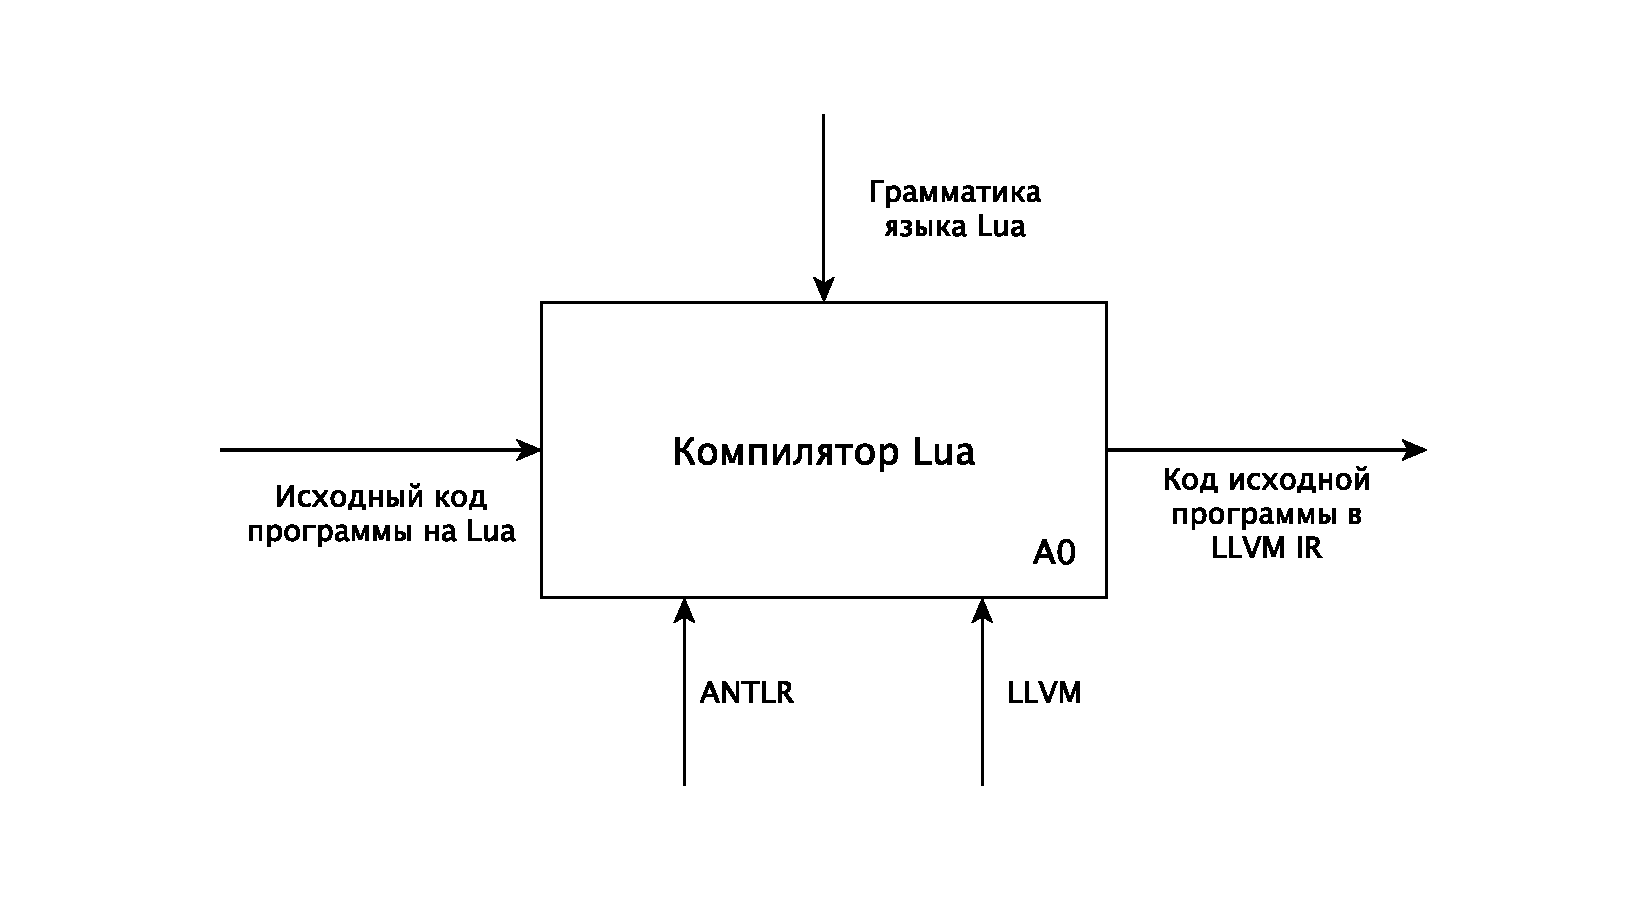
\includegraphics[width=0.8\linewidth]{./images/idef.pdf}}
	\caption{Концептуальная модель разрабатываемого компилятора в нотации IDEF0}
	\label{idef0}
   \end{figure}

\section{Язык Lua}

Lua~---~встраиваемый язык сценариев. 
Он поддерживает процедурное программирование, объектно-ориентированное программирование, функциональное программирование, программирование, управляемое данными, и описание данных.
Lua сочетает в себе процедурный синтаксис с конструкциями описания данных, основанными на ассоциативных массивах и расширяемой семантике. 
Lua динамически типизирован, работает путем интерпретации байт-кода с помощью виртуальной машины на основе регистров и имеет автоматическое управление памятью с инкрементальной сборкой мусора, что делает его идеальным для конфигурирования, написания сценариев и быстрого прототипирования.

Грамматика приведена в Приложении А.

\section{Лексический и синтаксический анализаторы}

Лексический и синтаксический анализаторы в данной работе генерируются с помощью ANTLR. 
На вход поступает грамматика языка в формате ANTLR4.

В результате работы создаются файлы, содержащие классы лексера и парсера, а также вспомогательные файлы и классы для их работы. 
Также генерируются шаблоны классов для обхода дерева разбора, которое получается в результате работы парсера.
На вход лексера подаётся текст программы, преобразованный в поток символов. 
На выходе получается поток токенов, который затем подаётся на вход парсера.
Результатом его работы является дерево разбора.
Ошибки, возникающие в ходе работы лексера и парсера, выводятся в стандартный поток ввода-вывода.

\section{Семантический анализ}

Абстрактное синтаксическое дерево можно обойти двумя способами: применяя паттерн Listener или Visitor.
Listener позволяет обходить дерево в глубину и вызывает обработчики соответствующих событий при входе и выходе из узла дерева.
Visitor предоставляет возможность более гибко обходить построенное дерево и решить, какие узлы и в каком порядке нужно посетить. 
Таким образом, для каждого узла реализуется метод его посещения. Обход начинается с точки входа в программу.
В данной работе используется паттерн Visitor.

\section{Вывод}

В текущем разделе была представлена концептуальная модель в нотации IDEF0, приведена грамматика языка Lua, описаны принципы работы лексического и синтаксического анализаторов и идея семантического анализа.
